\section{System Design Overview}

A search engine comprises two components: a \emph{crawler} that collects data and an \emph{indexer\slash search component} that retrieves and displays results. To parallelize development, one team member built the crawler while the other implemented the search interface.

\subsection{Crawler}

We both started by crawling our own universities, mine being INSA Lyon in France. I used \textbf{Selenium} to send requests and \textbf{BeautifulSoup} to parse the HTML content. \textbf{Selenium} was used because INSA Lyon's website is a single page application that only allows users to search people by name, as shown in \autoref{fig:insa_results_page}. This means that we cannot scrape the entire list of people from the website, but we can search for them by name. To collect all professor listings, we queried every two letter combination (``aa,'' ``ab,'' …, ``zz'') with a polite rate limit, saved results to CSV, and filtered out duplicates, students, and staff.

\begin{figure}[ht]
	\centering
	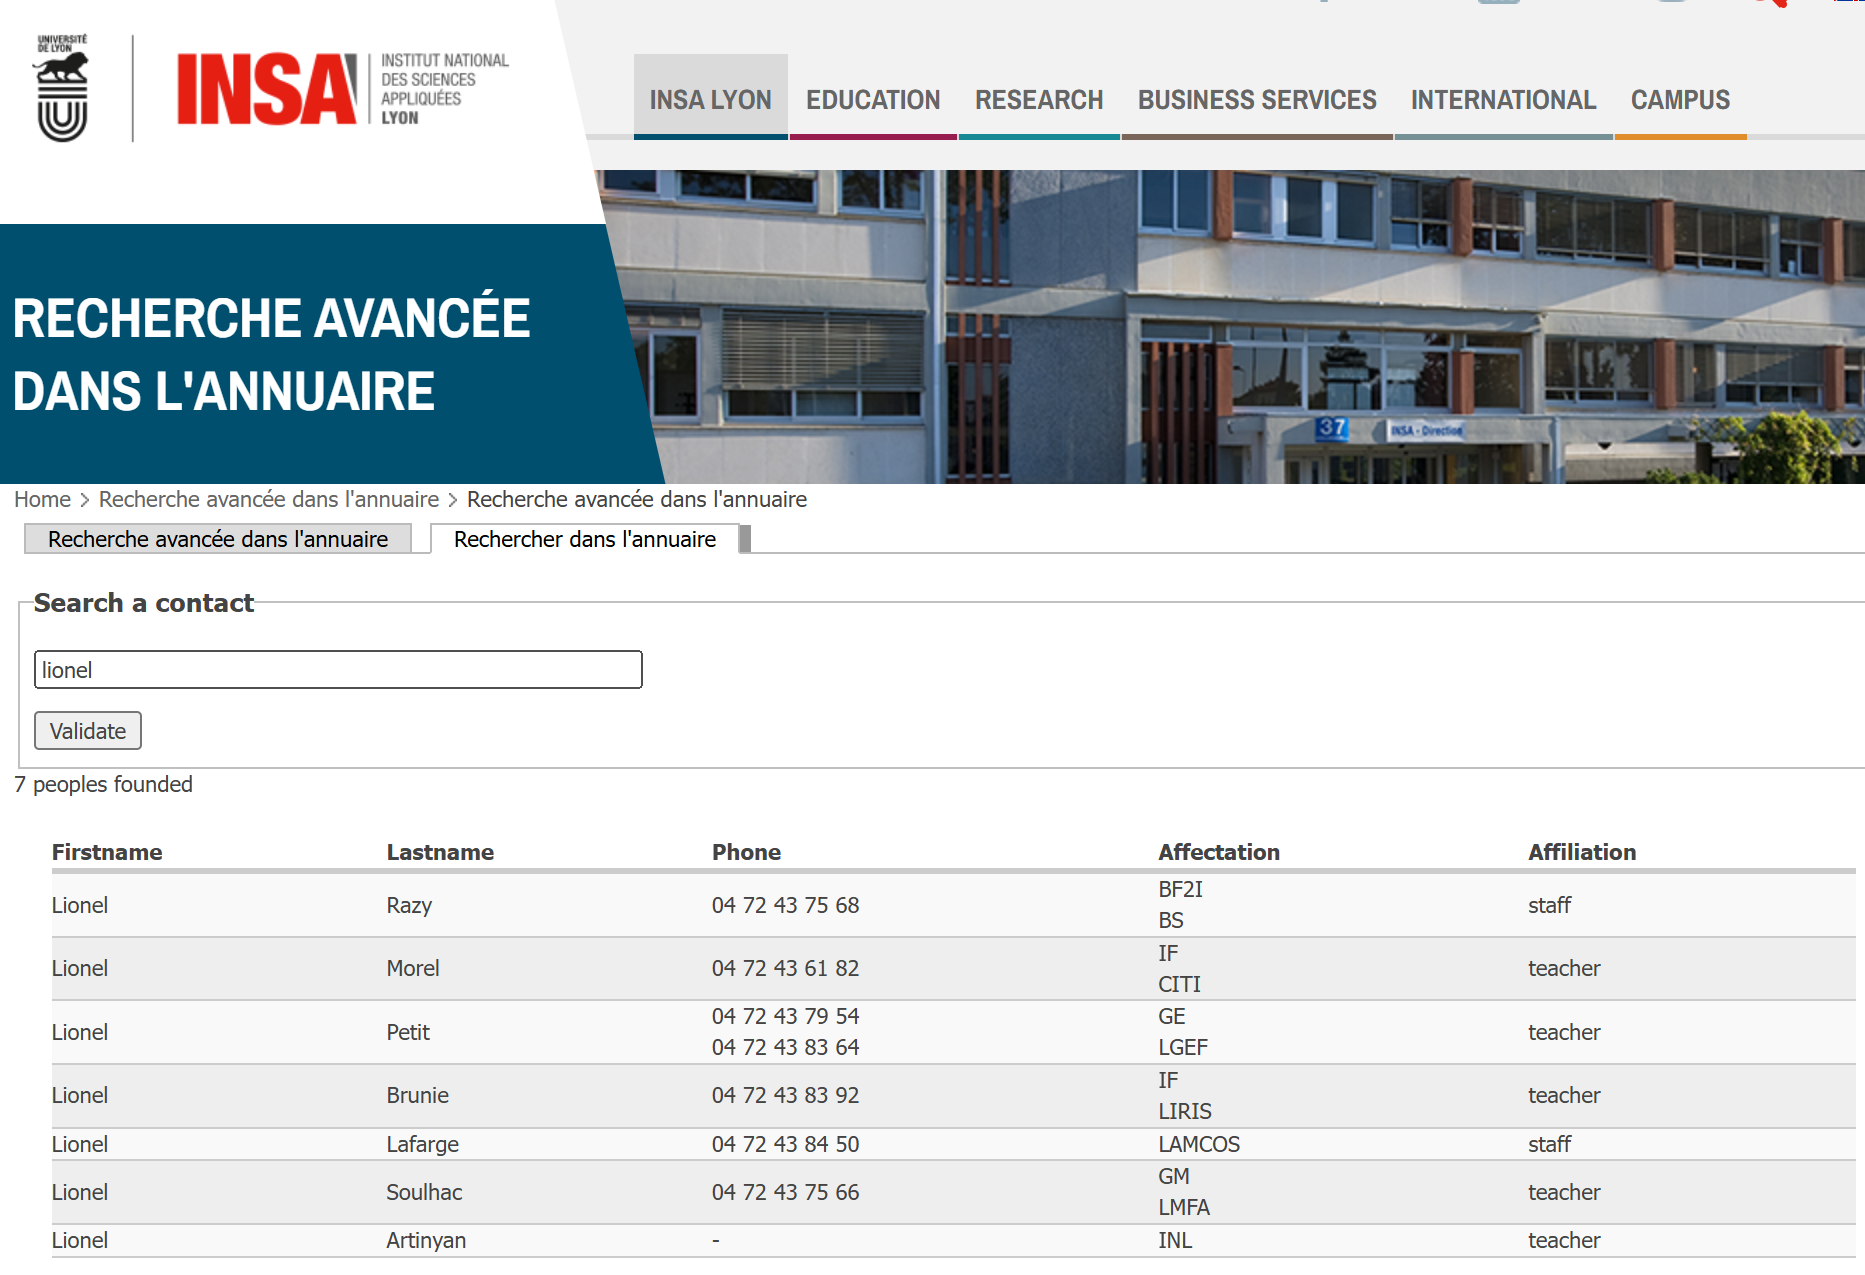
\includegraphics[width=0.7\textwidth]{insa-results-page.png}
	\caption{INSA Lyon's Results Page}
	\label{fig:insa_results_page}
\end{figure}

Now that I had data from my university, I started designing the layout of the search engine. I wanted a simple and clean design.

\subsection{Search Engine}

I started by looking at different people search engines: LinkedIn, Instagram, Facebook, etc. I wanted to see how they display the results and what information they show. I also looked at different search engines such as Google to see how they display the results. Since our data is professor-centric, each result displays name, title, university, department, and—if available—a profile picture. We modeled Sorgle's layout on LinkedIn's search results (\autoref{fig:linkedin_results_page}~\cite{linkedin2025} vs \autoref{fig:sorgle_results_page}) and profile page (\autoref{fig:linkedin_profile_page}~\cite{linkedin2025} vs. \autoref{fig:sorgle_profile_page}).

\begin{figure}[ht]
	\centering
	\begin{minipage}{0.48\textwidth}
		\centering
		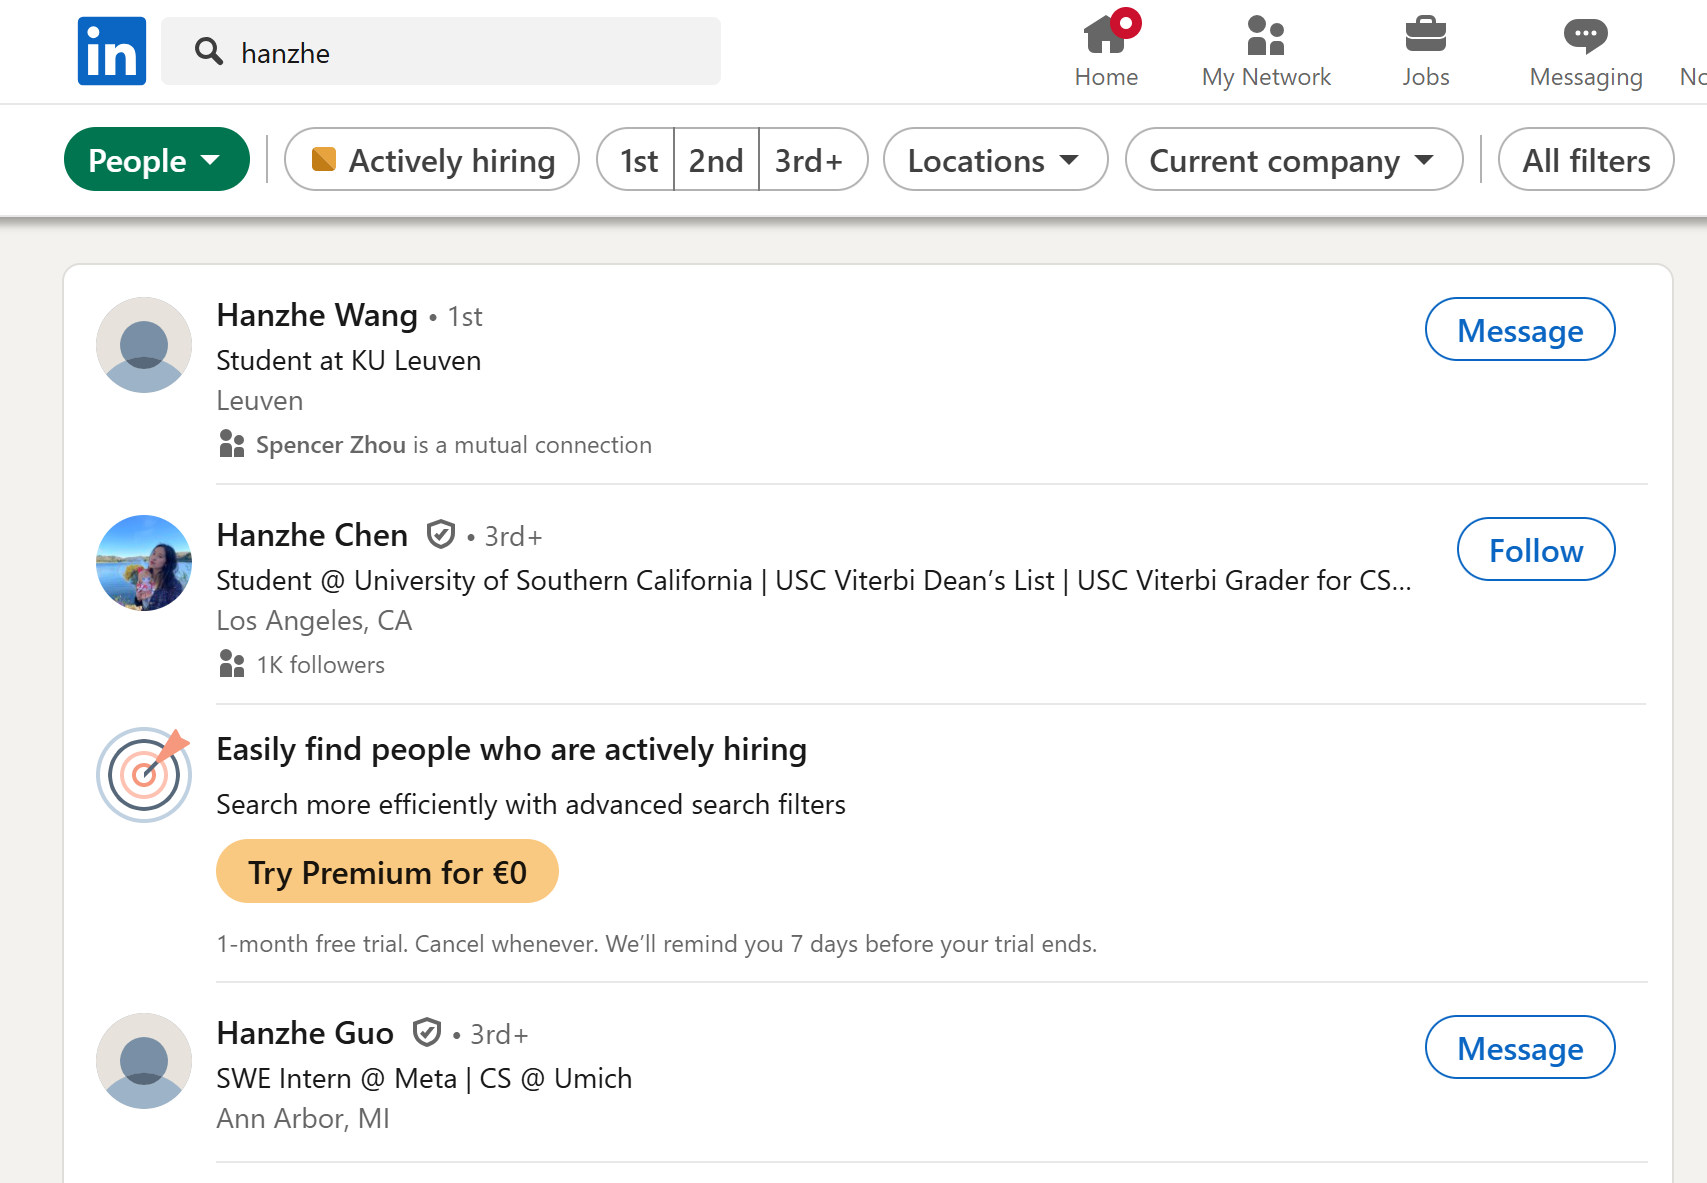
\includegraphics[width=\textwidth]{linkedin-results-page.png}
		\caption{LinkedIn Results Page \cite{linkedin2025}}
		\label{fig:linkedin_results_page}
	\end{minipage}\hfill
	\begin{minipage}{0.48\textwidth}
		\centering
		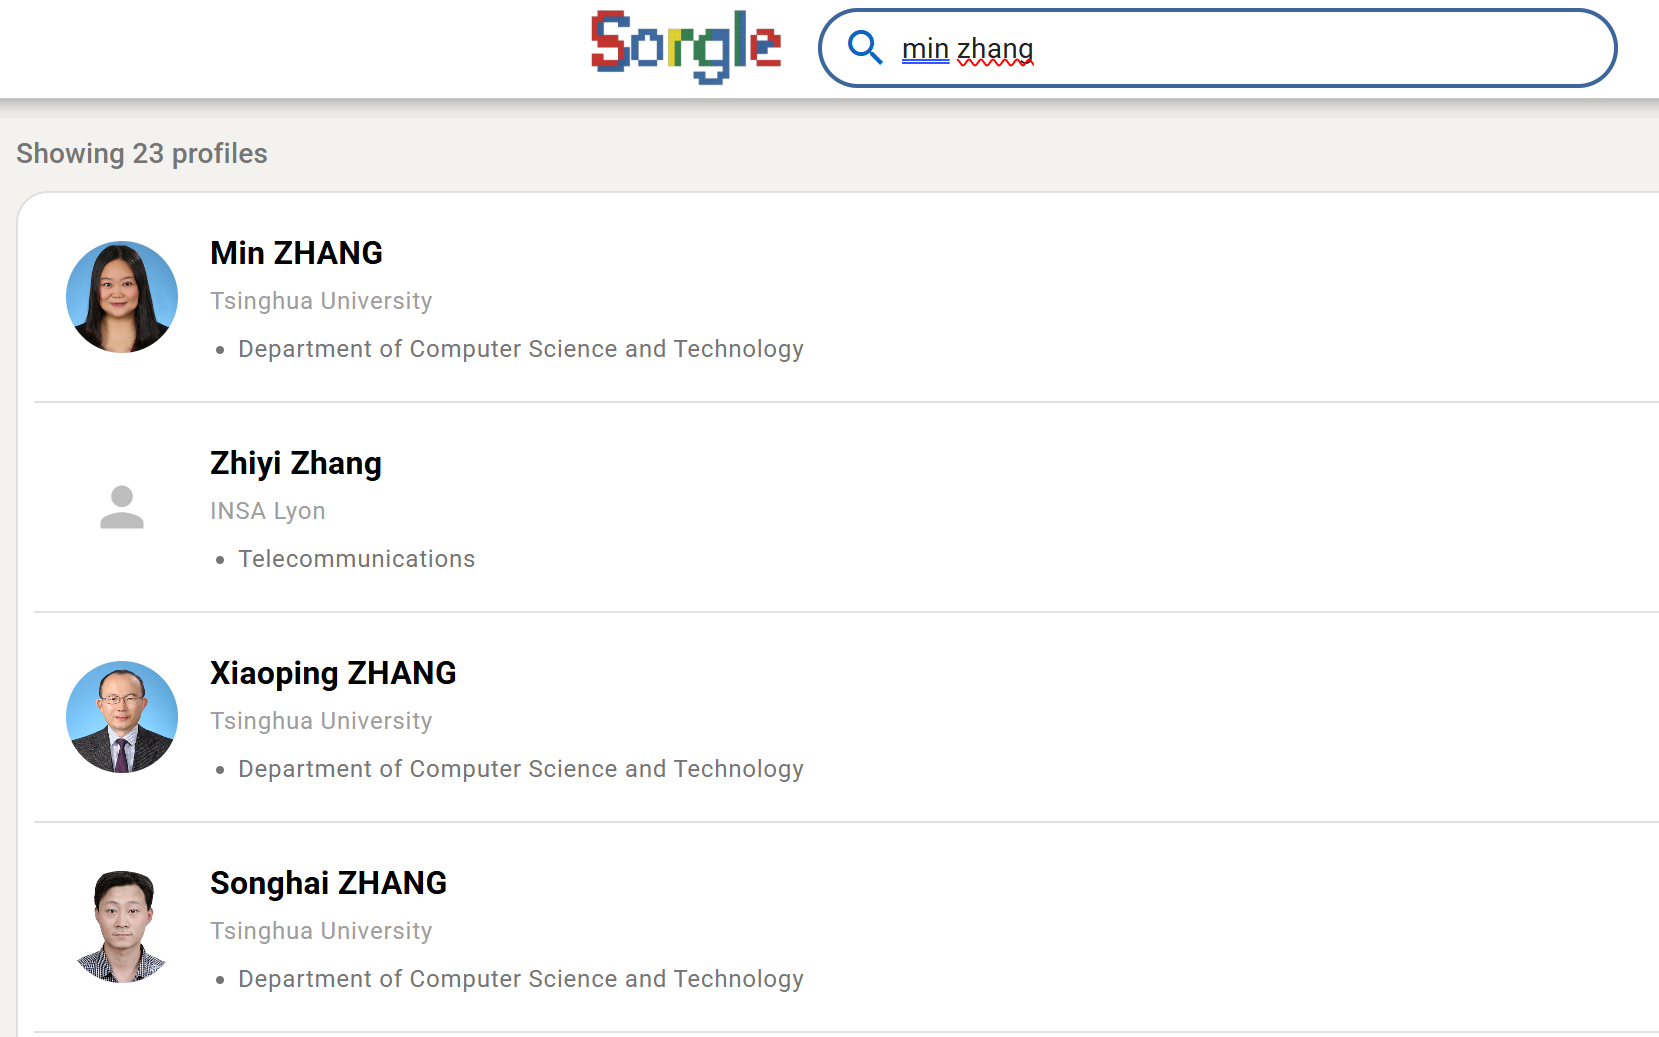
\includegraphics[width=\textwidth]{sorgle-results-page.png}
		\caption{Sorgle Results Page}
		\label{fig:sorgle_results_page}
	\end{minipage}
\end{figure}

\begin{figure}[ht]
	\centering
	\begin{minipage}{0.48\textwidth}
		\centering
		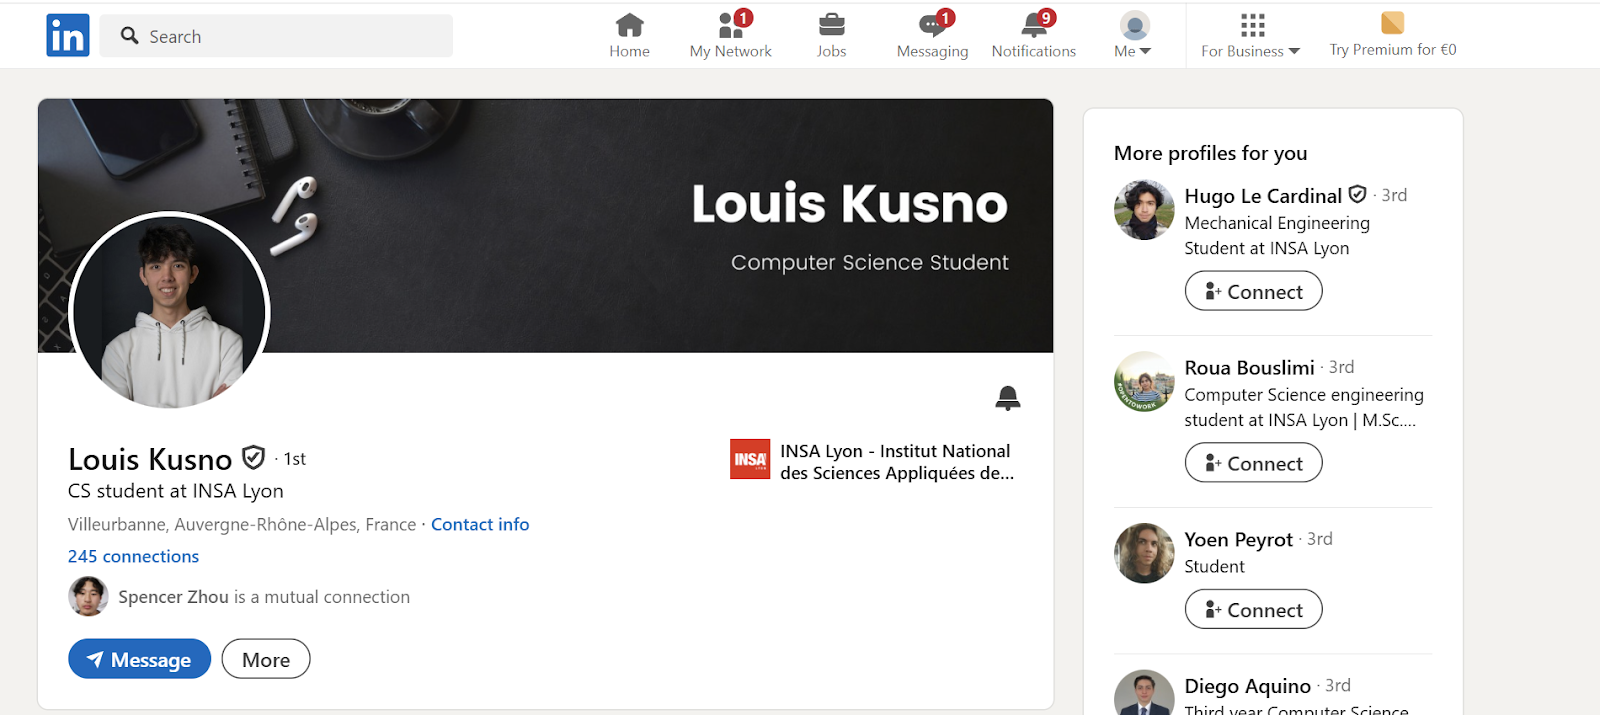
\includegraphics[width=\textwidth]{linkedin-profile-page.png}
		\caption{LinkedIn Profile Page \cite{linkedin2025}}
		\label{fig:linkedin_profile_page}
	\end{minipage}\hfill
	\begin{minipage}{0.48\textwidth}
		\centering
		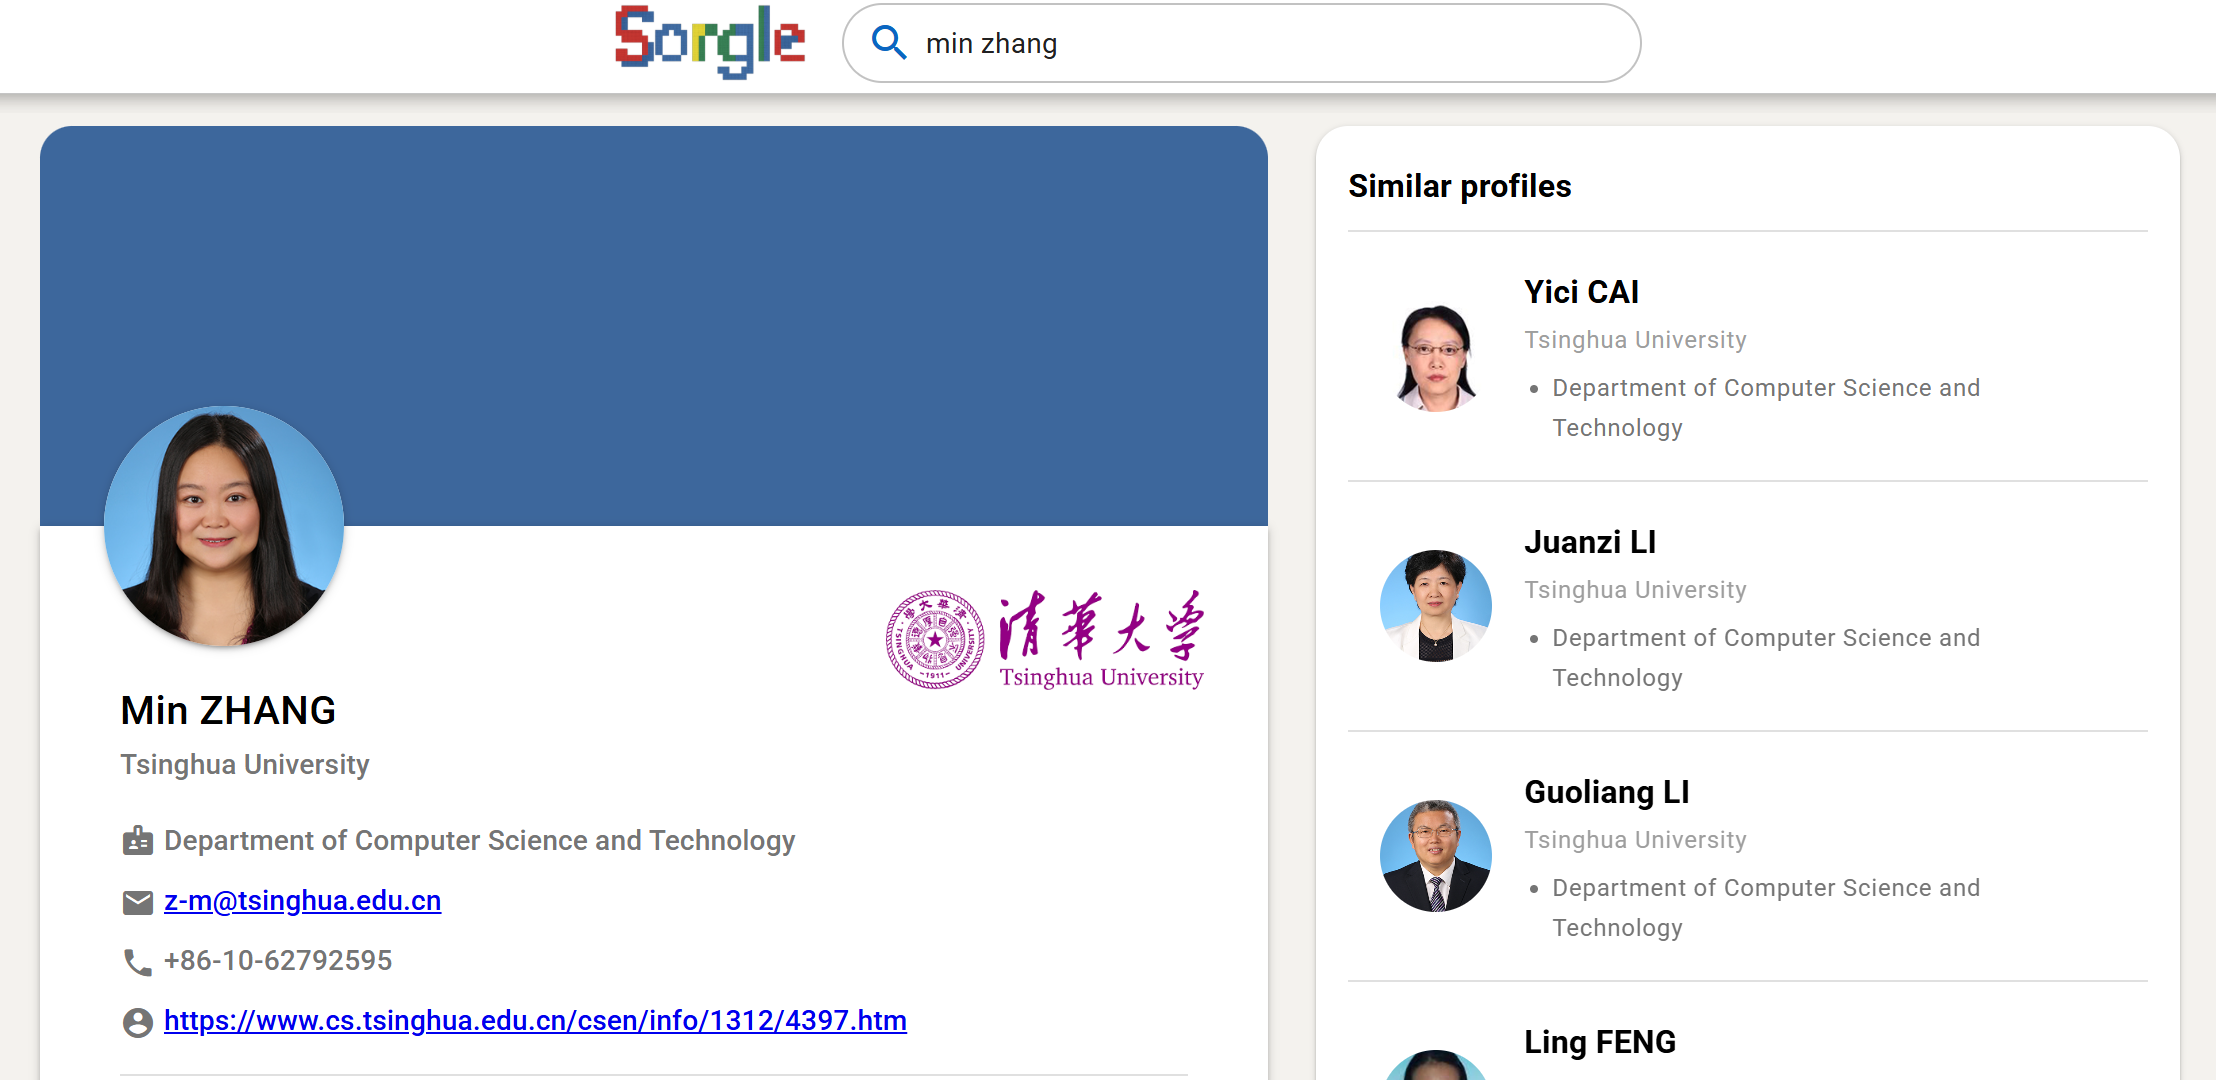
\includegraphics[width=\textwidth]{sorgle-profile-page.png}
		\caption{Sorgle Profile Page}
		\label{fig:sorgle_profile_page}
	\end{minipage}
\end{figure}

Results pages feature a top aligned search bar with concise entries (name, university, department) and a light mode color scheme inspired by LinkedIn. Even thought I set all my apps to dark mode, I think that light mode allows for a better looking website. Profile pages display all scraped fields - name, university, department, profile picture, phone, functions, ORCID, and bio - using icons to avoid clutter. We also added a \emph{similar profiles} sidebar to utilize empty space and improve user retention.

Finally, Sorgle's homepage mimics Google's minimalistic design to maintain simplicity and consistency.

\begin{figure}[ht]
	\centering
	\begin{minipage}{0.48\textwidth}
		\centering
		
\includegraphics[width=\textwidth]{google-main-page.png}
		\caption{Google Main Page \cite{google2025}}
		\label{fig:google_main_page}
	\end{minipage}\hfill
	\begin{minipage}{0.48\textwidth}
		\centering
		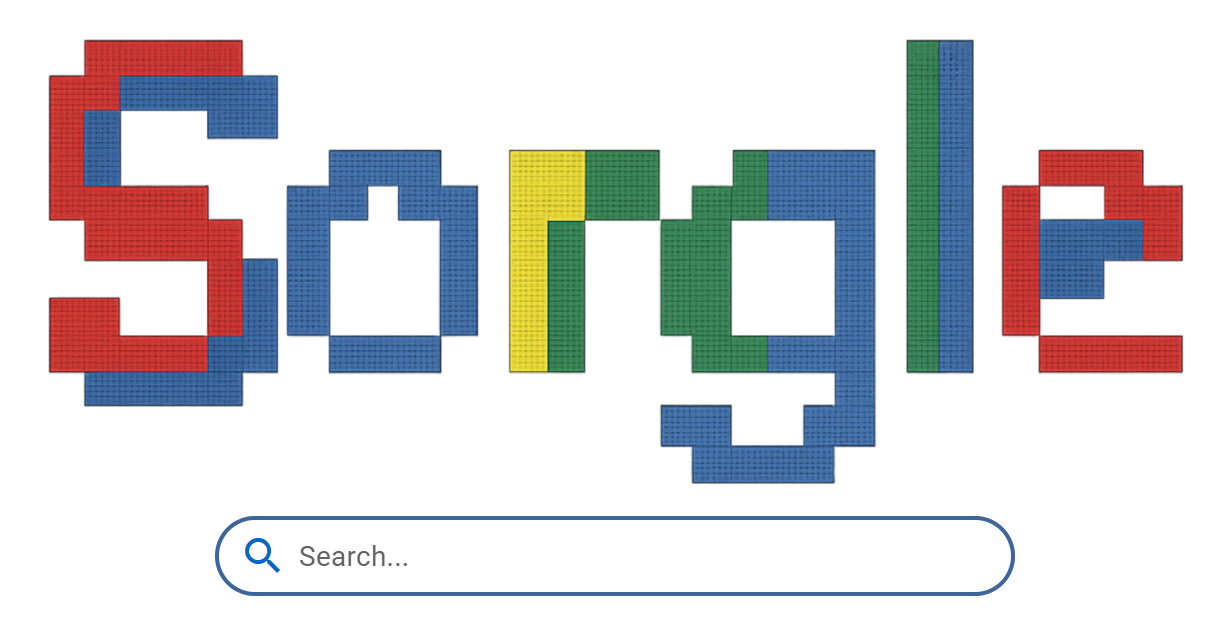
\includegraphics[width=\textwidth]{sorgle-main-page.png}
		\caption{Sorgle Main Page}
		\label{fig:sorgle_main_page}
	\end{minipage}
\end{figure}